\documentclass[10pt,a4paper]{extarticle}
\usepackage[latin1]{inputenc}
\usepackage{amsmath}
\usepackage{microtype}
\usepackage[none]{hyphenat}
\usepackage{verbatim}
\usepackage{amsfonts}
\usepackage{amssymb}
\usepackage{enumitem}
\renewcommand{\familydefault}{\sfdefault}
\usepackage{mathpazo}
\renewcommand{\rmdefault}{put}
\usepackage{enumitem}
\usepackage[dvipsnames,svgnames]{xcolor}
\usepackage{tkz-euclide}
\usetkzobj{all}
\usepackage{graphicx}
\usepackage{subcaption}
\usepackage{tikz} 	
\usepackage{adjustbox}
\usepackage{multicol}
\usepackage{lipsum}
\usepackage[left=0.7cm,right=1cm,top=1cm,bottom=1.5cm]{geometry}
\usepackage{cancel} \usepackage{xcolor}
\usepackage{tcolorbox}
\usetikzlibrary{decorations.pathmorphing,patterns}
\usetikzlibrary{decorations.pathreplacing,calc}
 \newcommand\coret[2][red]{\renewcommand\CancelColor{\color{#1}}\cancel{#2}}
\SetLabelAlign{Center}{\hfil\makebox[1.0em]{#1}\hfil}

%%_------= solusi


% Set this =0 to hide, =1 to show

% Set this =0 to hide, =1 to show
\newtcolorbox{mybox}[1][] { colframe = blue!10, colback = blue!3,boxsep=0pt,left=0.2em, coltitle = blue!20!black, title = \textbf{jawab}, #1, } 

%---------- kunci (jika 1 ) muncul
\def\tampilkunci{1}
\newcommand{\hide}[1]{\ifnum\tampilkunci=1
%
\begin{mybox}
 #1
\end{mybox}
%
\vspace{\baselineskip}\fi}



\newcommand*\cicled[1]{\tikz[baseline=(char.base)]{\node[white, shape=circle, fill=red!80,draw,inner sep=0.5pt](char){#1};}}

\newcommand*\kunci[1]{\ifnum\tampilkunci=1
%
\tikz[baseline=(char.base)]{\node[red, shape=circle,draw,inner sep=0.5pt,xshift=2pt](char){#1};}\stepcounter{enumii}
\fi\ifnum\tampilkunci=0
%
\hspace{3pt}#1\stepcounter{enumii}
%
\fi}

\newcommand*\silang[1]{\tikz[baseline=(char.base)]{
\draw[red,thick](-0.2,-0.20)--(0.2,0.2);
\draw[red,thick](-0.2,0.20)--(0.2,-0.2);
\node[black](char){#1};
}}

\newcommand*\centang[1]{\tikz[baseline=(char.base)]{
\draw[red, very thick](-0.2,0.1)--(-0.1,0)--(0.2,0.3);
\node(char){#1};
}}

\newcommand*\merah[1]{
\textcolor{red}{#1}}
\newcommand*\pilgan[1]{
\begin{enumerate}[label=\Alph*., itemsep=0pt,topsep=0pt,leftmargin=*,align=Center] #1 
\end{enumerate}}
\newcommand*\pernyataan[1]{
\begin{enumerate}[label=(\arabic*), itemsep=0pt,topsep=0pt,leftmargin=*] #1 
\end{enumerate}}

\newcommand{\pilgani}[1]{                            \vspace{-0.3cm}\begin{multicols}{2}
 \begin{enumerate}[label=\Alph*., itemsep=0pt,topsep=0pt,leftmargin=*,align=Center]#1                     \end{enumerate}
 \phantom{ini cuma sapi, wedus, dan ayam}
 \end{multicols}}


\begin{document}


 \textbf{Alat Optik} \phantom{ini nama siswa yang aaamengerjakan soal kuis ini }  

\begin{multicols*}{2}\raggedcolumns
\textbf{A. Mata}\\
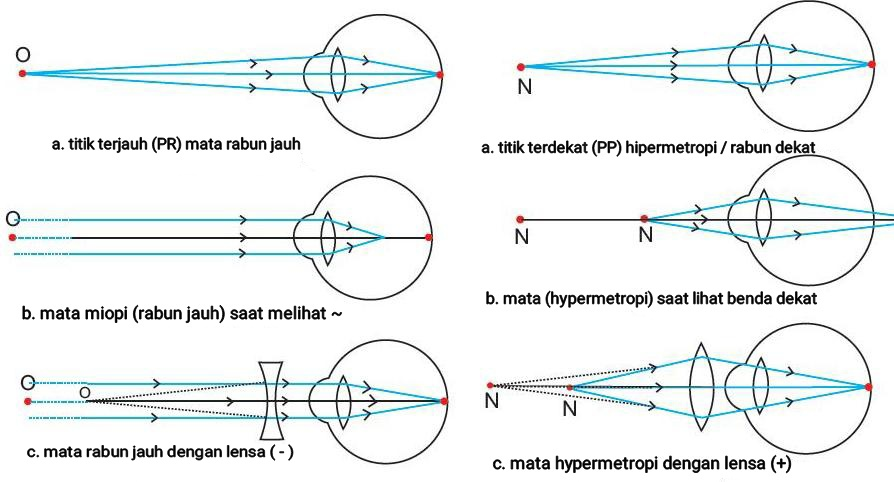
\includegraphics[width=9cm]{pic/mata} \\
\textbf{Mata Rabun Jauh}\\
Mata normal seharusnya dapat melihat dengan jarak tak hingga $\infty$, sedangkan pada mata rabun jauh, hanya terbatas melihat sampai jarak terjauh (Punctum Remotum) PR. Bayangan $s'$ bentuknya tegak, sehingga pasti sifatnya maya (-)\\
\vspace{0.7cm}
\textbf{rumus rabun jauh}
\vspace{-0.7cm}
\begin{align*}
\frac{100}{f(cm)} &= \frac{100}{s}+\frac{100}{s'}\\
\frac{100}{f} &= \frac{100}{\infty} -\frac{100}{PR}\\
\frac{100}{f} &= -\frac{100}{PR}
\end{align*}


\textbf{kuat lensa / power }
\begin{align*}
P &= \frac{1 }{f\text{(m)}}=\frac{100}{f\text{ (cm)}}
\end{align*}
\vspace{0.8cm}

\begin{enumerate}

\item Aminah ingin membelikan kacamata untuk temannya yang hanya dapat melihat benda terjauh pada jarak 3 meter. Jenis kacamata apakah yang harus dibeli Aminah .
\pilgani{
	\item -1/3 D
	\item -2/3 D
	\item +2/3 D
	\item +1/3 D
	\item 1 D }
\vspace{3cm}

\item Seseorang bermata miopi hanya dapat melihat benda yang jelas paling jauh jaraknya 50 cm. Kekuatan lensa kacamata yang harus digunakan agar orang tersebut dapat melihat jelas pada benda-benda jauh adalah . . .
\pilgani{
	\item 2 Dioptri
	\item 4 Dioptri
	\item 1 Dioptri
	\item -4 Dioptri
	\item -2 Dioptri }
\vspace{3cm}

\textbf{Mata Rabun Dekat}\\
Mata rabun dekat tidak bisa melihat terlalu dekat. Orang normal rata-rata bisa melihat hingga 25 cm. Saat menderita rabun dekat, jarak yang bisa dilihat lebih dari 25 cm, misal 40 cm, 50 cm, 100 cm. Sehingga biasanya orang yang rabun dekat menjauhkan buku saat membaca. Jarak dekat yang masih mampu dilihat ini disebut Punctum Proximum (PP). Fungsi kacamata pada rabun dekat adalah melihat benda dekat ($Sn$=25 cm) sebagai $s$ dan PP sebagai bayangan $s'$ yang tegak, sehingga maya $(-)$\\
\vspace{1cm}
\textbf{rumus rabun dekat}
\vspace{-0.7cm}
\begin{align*}
\frac{100}{f(cm)} &= \frac{100}{s}+\frac{100}{s'}\\
\frac{100}{f} &= \frac{100}{sn} - \frac{100}{PP}
\end{align*}

\item Seseorang menderita rabun dekat dengan titik dekat 50 cm ingin membaca pada jarak baca normal. Jenis lensa kacamata yang harus digunakan dan jarak fokusnya adalah 
\pilgan{
	\item cembung dengan fokus 50 cm
	\item cekung dengan fokus 33,3 cm
	\item rangkap dengan fokus 25 cm
	\item cembung dengan fokus 33,3 cm
	\item cekung dengan fokus 50 cm }
\vspace{2cm}

\item Seseorang penderita hipermetropi memiliki titik dekat 50 cm hendak membaca pada jarak baca normal. Orang tersebut memerlukan kacamata berkekuatan . . . 
\pilgani{
	\item -2 Dioptri
	\item -1/2 Dioptri
	\item +1/2 Dioptri
	\item +2 Dioptri
	\item +4 Dioptri }
\vspace{2cm}


\item Seorang penderita presbiopi mempunyai titik dekat 50 cm dan titik jauh 2,5 m. Kekuatan lensa yang harus digunakan adalah . . 
\pilgani{
	\item 2 D dan -0,4 D
	\item 2 D dan 0,4 D
	\item 2,5 D dan -2 D
	\item 4 D dan -2 D
	\item 4 D dan -4 D }
\vspace{5cm}


\textbf{LUP /  Kaca Pembesar}\\
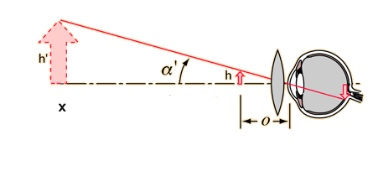
\includegraphics[width=8cm]{pic/lup}

Kaca pembesar menggunakan satu lensa cembung, untuk menghasilkan perbesaran tertentu. Bayangan yang dibentuk pasti tegak, sehingga bayangannya maya. Pada lup, yang diperlukan adalah perbesarannya atau Magnification. 

Saat bayangan di tak hingga $\infty$, mata tidak berakomodasi, sedangkan saat melihat di titik terdekat ($Sn = 25$ cm) mata berakomodasi maksimum. Titik akomodasi disebut $x$

\textbf{rumus lup}
\begin{align*}
M &= \frac{sn}{f} + \frac{sn}{x}
\end{align*}

\item Sebuah lup mempunyai jarak fokus 5 cm dipakai melihat sebuah benda kecil yang berjarak 5 cm dari lup. Jika dilihat dengna mata akomodasi, maka perbesaran anguler dari lup adalah . . .
\pilgani{
	\item 2
	\item 4
	\item 25/6
	\item 5
	\item 25/4}
\vspace{2cm}


\item Seorang siswa berpenglihatan normal (jarak baca 25 cm) mengamati benda kecil melalui lup dengan akomodasi maksimum. Jika benda itu 10 cm di depan lup, maka . . .
\pernyataan{
	\item jarak fokus lensa lup 16$\frac{2}{3}$
	\item kekuatan lensa lup 6 D
	\item perbesaran bayangan 2,5 kali
	\item perbesaran bayangan menjadi 2 kali perbesaran tanpa akomodasi
}
\vspace{2cm}

\item Sebuah lup dengan panjang fokus lensa 5 cm digunakan untuk melihat sebuah benda kecil. Dengan asumsi titik dekat normal adalah 25 cm, tentukan perbesaran lup untuk mata pengamat jika berakomodasi maksimum . . .
\pilgani{
	\item 4 kali
	\item 5 kali
	\item 6 kali
	\item 12 kali
	\item 20 kali }
\vspace{2cm}

\item Sebuah lup dengan panjang fokus lensa 5 cm digunakan untuk melihat sebuah benda kecil. Dengan asumsi titik dekat normal adalah 25 cm, tentukan perbesaran lup untuk mata pengamat jika tidak berakomodasi . . .
\pilgani{
	\item 4 kali
	\item 5 kali
	\item 6 kali
	\item 12 kali
	\item 20 kali }
\vspace{2cm}

\item Sebuah lup dengan panjang fokus lensa 5 cm digunakan untuk melihat sebuah benda kecil. Dengan asumsi titik dekat normal adalah 25 cm, tentukan perbesaran lup untuk mata pengamat jika berakomodasi pada jarak 20 cm . . .
\pilgani{
	\item 1,25 kali
	\item 2,50 kali
	\item 6,25 kali
	\item 8,12 kali
	\item 10,25 kali }
\vspace{2cm}

\textbf{Microskop}\\
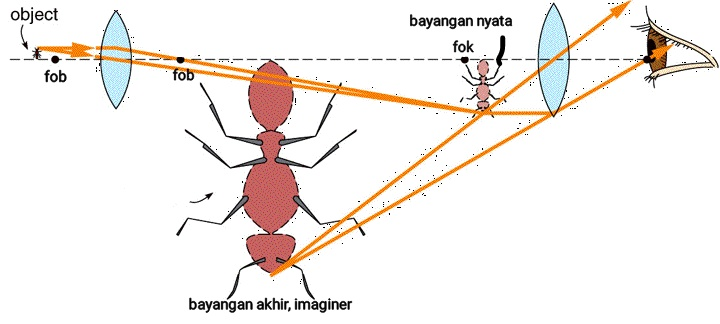
\includegraphics[width=8cm]{pic/mikroskop}

Mikroskop adalah alat untuk memperbesar bayangan pada benda yang sangat kecil. Mikroskop terdiri dari dua benda, yakni lensa objektif dan lensa okuler. Perbesaran pada lensa okuler sama seperti pada lup.
\begin{align*}
M &= M_{ob} \times M_{ok} =\frac{s'_{ob}}{s_{ob}}\times \left ( \frac{sn}{f_{ok}}+\frac{sn}{x}\right)
\end{align*}
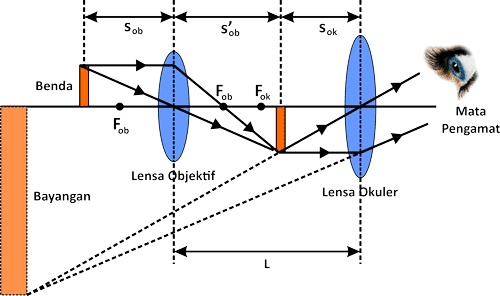
\includegraphics[width=8cm]{pic/mikroskop2}\\
Panjang mikroskop $d$
\begin{align*}
d&= s'_{ob} + s_{ok} \\
d &= s'_{ob} + f_{ok} \text{ saat TANPA akomodasi}
\end{align*}

\vspace{3cm}


\item Sebuah mikroskop mempunyai lensa objektif yang jarak titik apinya 2 cm. Sebuah objek diletakkan 2,2 cm di bawah objektif. Jika perbesaran okuler 10 kali, maka perbesaran mikroskop sama dengan . . . 
\pilgani{
	\item 300 kali
	\item 110 kali
	\item 220 kali
	\item 100 kali
	\item 200 kali}
\vspace{3cm}

\item Sebuah mikroskop mempunyai jarak fokus objektif 8 mm, dan jarak fokus okuler 60 mm. Jika preparat ditempatkan 10 mm di depan objektif dan mata melihat tanpa akomodasi, maka panjang tabung mikroskop tersebut adalah . . 
\pilgani{
	\item 100 cm
	\item 60 cm
	\item 40 cm
	\item 20 cm
	\item 10 cm }
\vspace{3cm}


\textbf{rumus Teropong}
\begin{align*}
M &= \frac{f_{ob}}{f_{ok}} \left( 1 +\frac{f_{ok}}{x}\right)
\end{align*}
Panjang Teropong $d$
\begin{align*}
d&=f_{ob} + s_{ok} \\
d &= f_{ob} + f_{ok} \text{ saat TANPA akomodasi}
\end{align*}

\item Teropong bintang dengan perbesaran anguler 10 kali. Bila jarak titik api objektifnya 50 cm, maka panjang teropong . . . 
\pilgani{
	\item 5 cm
	\item 35 cm
	\item 45 cm
	\item 50 cm
	\item 55 cm }
\vspace{3cm}

\item Sifat dan kedudukan bayangan yang dihasilkan oleh lensa objektif sebuah teropong bintang . . .
\pilgani{
	\item nyata, terbalik, tepat di titik fokus lensa objektif
	\item nyatak, tegak dan tepat di titik fokus lensa okuler
	\item nyata, tegak dan tepat di titik fokus lensa objektif
	\item maya, terbalik dan tepat di titik fokus lensa okuler
	\item maya, terbalik dan tepat di titik fokus lensa objektif
}
\vspace{2cm}

\item Sebuah teropong dipakai untuk melihat bintang yang menghasilkan perbesaran anguler 6 kali. Jarak fokus lensa objektif 30 cm, jarak fokus okulernya (mata tak berakomodasi) adalah . . .
\pilgani{
	\item 3,5 cm
	\item 5 cm
	\item 7 cm
	\item 10 cm
	\item 30 cm }
\vspace{3cm}

\item Sebuah teropong bintang memiliki jarak fokus objektif 75 cm dan jarak fokus okuler 5 cm. Perbesaran sudut teleskop dengan mata berakomodasi pada jarak 50 cm adalah . . .
\pilgani{
	\item 9 kali
	\item 18 kali
	\item 20 kali
	\item 36 kali
	\item 45 kali }

\item Sebuah teropong bintang memiliki panjang fokus lensa okuler 15 mm. Saat meneropong objek langit, citranya akan nampak jelas ketika jarak antara objektif dan okuler sebesar 945 mm. Jika diinginkan perbesaran menjadi 310 kali, maka lensa okuler tersebut harus diganti dengan okuler lain dengan panjang fokus . . . 
\pilgani{
	\item 3 mm
	\item 5 mm
	\item 10 mm
	\item 20 mm
	\item 25 mm
}
\vspace{3cm}


\item Seorang tukang reparasi jam tangan menggunakan  sebuah lensa lup (kaca pembesar)  untuk melihat bagian-bagian mesin jam. Saat digunakan sesuai fungsinya bayangan yang dihasilkan lensa lup tersebut  memiliki sifat . . .
\pilgani{
	\item Maya, terbalik, diperkecil
	\item Maya, tegak, diperbesar
	\item Nyata, terbalik, diperbesar
	\item Nyata, tegak, diperbesar
	\item Nyata, tegak, diperkecil
}
\vspace{2cm}

\item Sebuah lensa berjarak fokus 5 cm digunakan sebagai lup. Jika mata normal menggunakan lup tersebut dengan berakomodasi maksimum, maka perbesaran anguler lup adalah . . . 
\pilgani{
	\item 3 kali
	\item 4 kali
	\item 5 kali
	\item 6 kali
	\item 8 kali }
\vspace{2cm}

\item Seorang anak menggunakan sebuah lup untuk melihat sebuah benda. Jika perbesaran yang diperoleh anak tersebut adalah 11 kali saat pengamatan dilakukan dengan mata berakomodasi maksimum maka fokus lensa lup yang digunakan besarnya adalah . . . (sn = 30 cm)
\pilgani{
	\item 2 cm
	\item 3 cm
	\item 4 cm
	\item 5 cm
	\item 6 cm }
\vspace{2cm}

\item Sebuah lensa berjarak fokus 4 cm digunakan sebagai lup. Agar mata melihat tanpa berakomodasi, maka letak benda tersebut dari lup adalah . . .
\pilgani{
	\item 2 cm
	\item 3 cm
	\item 4 cm
	\item 6 cm
	\item 8 cm
}
\vspace{2cm}

\item Amatilah diagram pembentukan bayangan oleh mikroskop berikut ini!\\
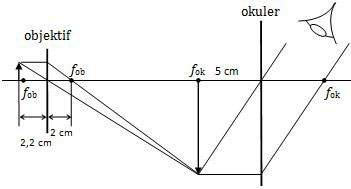
\includegraphics[width=7cm]{pic/bayangan-mikroskop2}\\
Jika berkas sinar yang keluar dari lensa okuler merupakan berkas sejajar dan mata yang mengamati berpenglihatan normal maka perbesaran mikroskop adalah . . .
\pilgani{
	\item 10 kali
	\item 18 kali
	\item 22 kali
	\item 30 kali
	\item 50 kali}\vspace{3cm}


\item Sebuah mikroskop memiliki jarak titik api obyektif 2,0 cm. Sebuah benda diletakkan di bawah objektif pada jarak 2,2 cm. Panjang mikroskop 24,5 cm dan pengamat dilakukan tanpa akomodasi. Jika pengamat bermata normal maka perbesaran total mikroskop bernilai . . .
\pilgani{	
	\item 20 kali
	\item 25 kali
	\item 50 kali
	\item 75 kali
	\item 100 kali
}
\vspace{4cm}

\item Ketika membaca, jarak terdekat yang dapat dilihat seroang kakek adalah 40 cm. Kekuatan lensa kacamata yang diperlukan kakek tersebut agar dapat melihat dengan normal adalah . . .
\pilgani{
	\item 3/2 dioptri
	\item 3/4 dioptri
	\item 2/3 dioptri
	\item 1/4 dioptri
	\item 4/3 dioptri}
\vspace{3cm}
%
%\item Lintasan berkas sinar ketika melalui sistem optik teropong bintang ditunjukkan seperti gambar. \\
%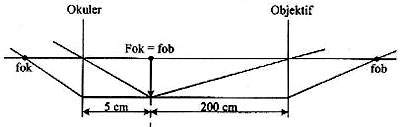
\includegraphics[width=8cm]{pic/teropong-bintang} \\
%Berdasarkan gambar di atas, perbesaran bayangan untuk mata tidak berakomodasi adalah . . .
%\pilgani{
%	\item 60 kali
%	\item 50 kali
%	\item 45 kali
%	\item 40 kali
%	\item 30 kali
%}
\vspace{3cm}
\item Perhatikan gambar pembentukan bayangan teropong berikut ini!\\
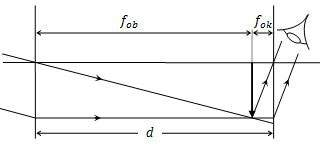
\includegraphics[width=7cm]{pic/bayangan-teropong}\\
Panjang teropong 110 cm dan jarak fokus lensa objektif 1 m. Perbesaran teropong untuk mata tidak berakomodasi adalah . . 
\pilgani{
	\item 20 kali
	\item 15 kali
	\item 10 kali
	\item 8 kali
	\item 5 kali }
\vspace{3cm}



\end{enumerate}
\end{multicols*}
\end{document}
